\chapter{Supplemental information for Chapter 2}

\begin{figure}
    \centering
    \makebox[\textwidth][c]{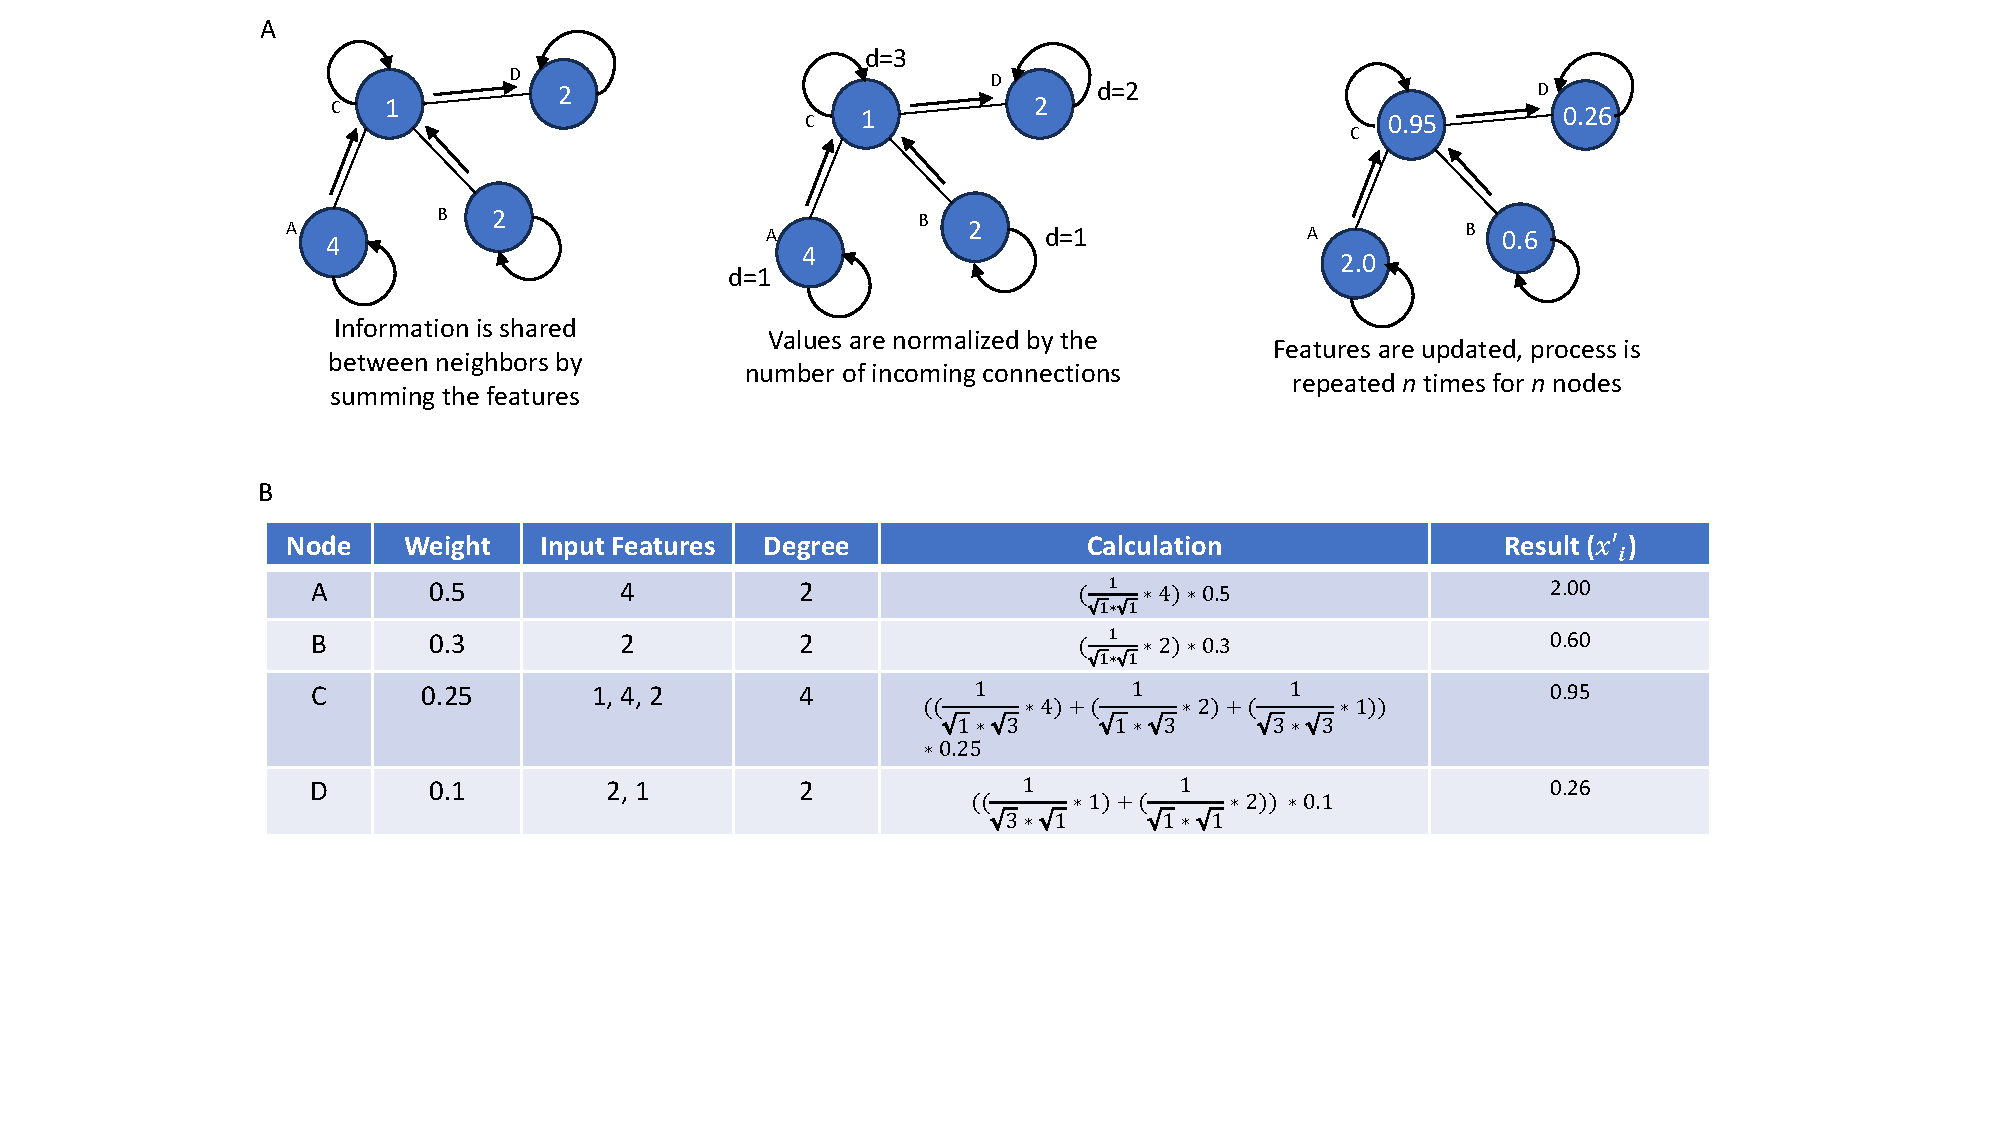
\includegraphics[width=1.2\textwidth]{figures/ap2/GCFigure_nolegend.pdf}}
    \caption[Diagram of graph convolution]{(A) Diagram of graph convolution and (B) resulting parameters and calculations to demonstrate graph convolution. In this example features are simplified to a vector containing a single learnable parameter, denoted by “weight”, and a single scalar value for initial input features.}
    \label{fig:enter-label}
\end{figure}

\begin{table}[htb]
\resizebox{\textwidth}{!}{%
\begin{tabular}{|l|l|l|l|l|}
\hline
\cellcolor[HTML]{F2F5F9}{\color[HTML]{2A2A2A} Task} & Selection & Introgression & Recombination & Demography \\ \hline
$N$ (effective pop size)                            & 10,000    & 233,863       & 14,714        & 10,000     \\ \hline
$\mu$ (mutation rate)                               & 1.2e-8    & 5e-9          & 1.5e-8        & 1.2e-9     \\ \hline
$\rho$ (recombination rate)                         & 1e-8      & 2e-8          & 1e-7          & 1e-8       \\ \hline
sample size                                         & 104       & 34            & 50            & 50         \\ \hline
$L$ (sequence length)                               & 110,000   & 10,000        & 20,000        & 1,500,000  \\ \hline
\end{tabular}%
}

\caption{Simulation and sampling parameterizations for each benchmark task.}

\end{table}